% ============================================================
% 电路基础实验 —— 实验四 一阶 RC 电路瞬态分析 预习报告
% ============================================================

\documentclass[12pt]{ctexart}

% --- 宏包 ---
\usepackage{graphicx}
\usepackage{amsmath}
\usepackage{float}
\usepackage{booktabs}
\usepackage{siunitx}
\usepackage{caption}
\usepackage{subcaption}
\usepackage{enumitem}

\sisetup{per-mode=symbol}

\graphicspath{{./figures/}{../requirements/extracted_images/word/media/}{./}}

\usepackage[left=2.5cm, right=2.5cm, top=2.5cm, bottom=2.5cm]{geometry}

\setlength{\jot}{6pt}
\linespread{1.5}
\setlist{nosep}

\begin{document}

% ==================== 封面 ====================
\thispagestyle{empty}

\begin{center}
    \LARGE\textbf{第4次实验\ 一阶 RC 电路瞬态分析预习报告}

    \vspace{1cm}
    \normalsize
    组名：第7组\quad 姓名：郭浩然\quad 学号：2024303980
\end{center}

\vspace{1cm}

% ==================== 正文 ====================

% (10) 实验目的
\section{实验目的}

\begin{enumerate}[label=\arabic*.]
    \item 学习函数信号发生器和示波器在瞬态电路测量中的基本使用方法。
    \item 掌握一阶 RC 电路零输入响应、零状态响应和全响应的基本概念。
    \item 理解一阶 RC 电路时间常数 \(\tau=RC\) 的物理意义和测量方法。
    \item 掌握 RC 微分电路和积分电路的基本工作原理及波形特征。
\end{enumerate}

% (80) 实验原理
\section{实验原理}

\subsection{一阶 RC 电路响应}

一阶 RC 电路由电阻和电容组成。由于电容电压不能突变，换路瞬间有
\begin{equation}
    u_C(0^+)=u_C(0^-).
\end{equation}
电路受到阶跃激励后，电容通过充电或放电逐渐达到新的稳态。其响应可分解为
\begin{align}
    \text{全响应} &= \text{零输入响应}+\text{零状态响应}, \\
    \text{全响应} &= \text{瞬态响应}+\text{稳态响应}.
\end{align}
电容电压的一般形式为
\begin{equation}
    u_C(t)=U_\infty+\left[u_C(0^+)-U_\infty\right]e^{-t/\tau},
    \label{eq:rc-general-response}
\end{equation}
其中，\(U_\infty\) 为稳态电压，\(\tau\) 为时间常数。

\subsection{时间常数与充放电规律}

一阶 RC 电路的时间常数为
\begin{equation}
    \tau=RC.
\end{equation}
本实验时间常数测量电路中，\(R=\SI{10}{\kilo\ohm}\)，\(C=\SI{0.01}{\micro\farad}\)，因此
\begin{equation}
    \tau=RC=\SI{10}{\kilo\ohm}\times\SI{0.01}{\micro\farad}
    =\SI{100}{\micro\second}.
    \label{eq:time-constant}
\end{equation}

电容放电对应零输入响应，若初始电压为 \(U_0\)，则
\begin{equation}
    u_C(t)=U_0 e^{-t/\tau}, \qquad
    u_C(\tau)=\frac{U_0}{e}\approx0.368U_0.
    \label{eq:zero-input}
\end{equation}
电容充电对应零状态响应，若阶跃输入终值为 \(U_0\)，则
\begin{equation}
    u_C(t)=U_0\left(1-e^{-t/\tau}\right), \qquad
    u_C(\tau)=U_0\left(1-\frac{1}{e}\right)\approx0.632U_0.
    \label{eq:zero-state}
\end{equation}
因此，可在示波器上分别由放电曲线的 \(0.368U_0\) 处或充电曲线的 \(0.632U_0\) 处读取时间常数。

\subsection{方波激励与积分、微分电路}

方波输入可看作连续的阶跃激励：上升沿对应电容充电，下降沿对应电容放电。当周期相对于时间常数足够大时，可观察到明显的指数上升和下降波形。

RC 电路还可实现近似积分或微分功能。积分电路通常取电容两端电压为输出，方波输入时输出呈平滑斜坡或近似三角波；微分电路通常取电阻两端电压为输出，方波跳变时输出正、负尖脉冲，稳态时输出趋近于零。

\subsection{Multisim 仿真电路}

时间常数测量电路如图~\ref{fig:rc-time-constant} 所示。示波器观察电容电压的充放电曲线，并由 \(0.632U_0\) 或 \(0.368U_0\) 对应时刻测量 \(\tau\)。

\begin{figure}[H]
    \centering
    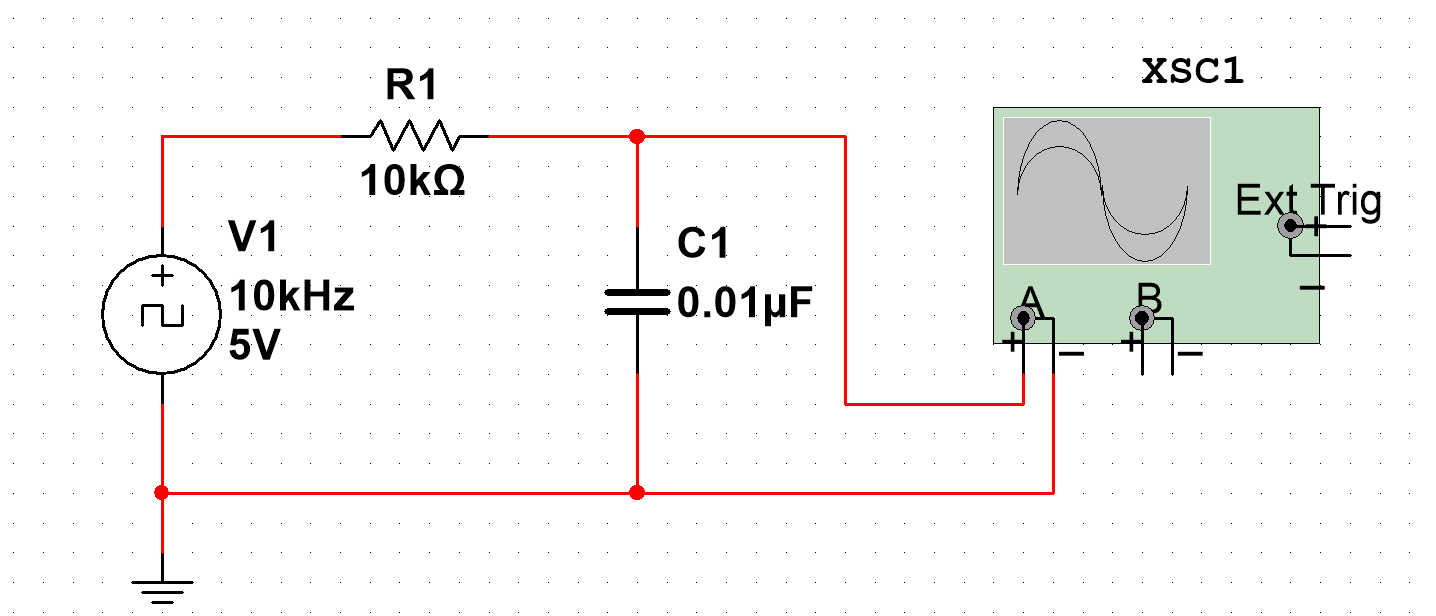
\includegraphics[width=0.82\textwidth]{rc_time_constant_multisim.png}
    \caption{时间常数测量 Multisim 仿真电路}
    \label{fig:rc-time-constant}
\end{figure}

积分电路如图~\ref{fig:rc-integrator} 所示，主要观察电容端输出的积分效果。

\begin{figure}[H]
    \centering
    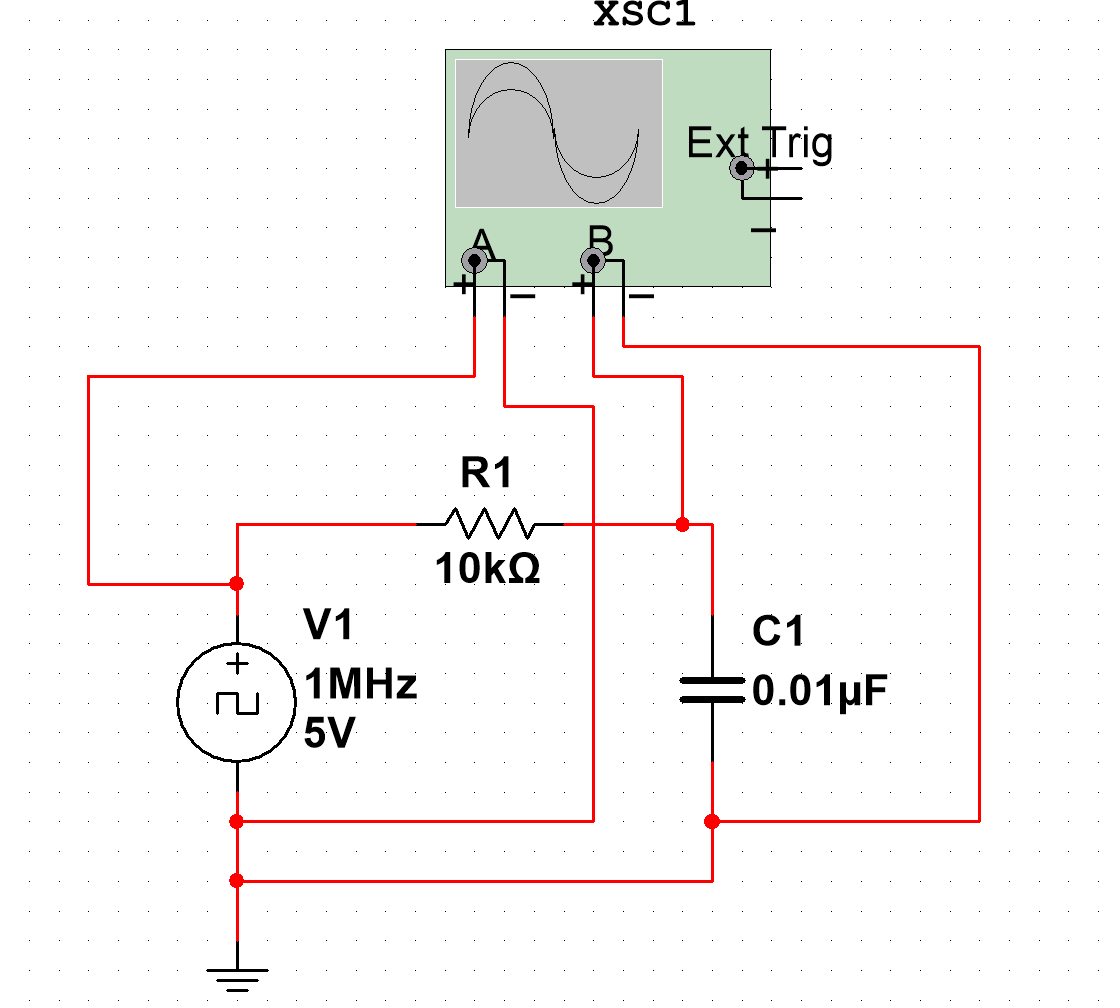
\includegraphics[width=0.68\textwidth]{rc_integrator_multisim.png}
    \caption{积分电路 Multisim 仿真电路}
    \label{fig:rc-integrator}
\end{figure}

微分电路如图~\ref{fig:rc-differentiator} 所示，主要观察电阻端输出的边沿尖脉冲响应。

\begin{figure}[H]
    \centering
    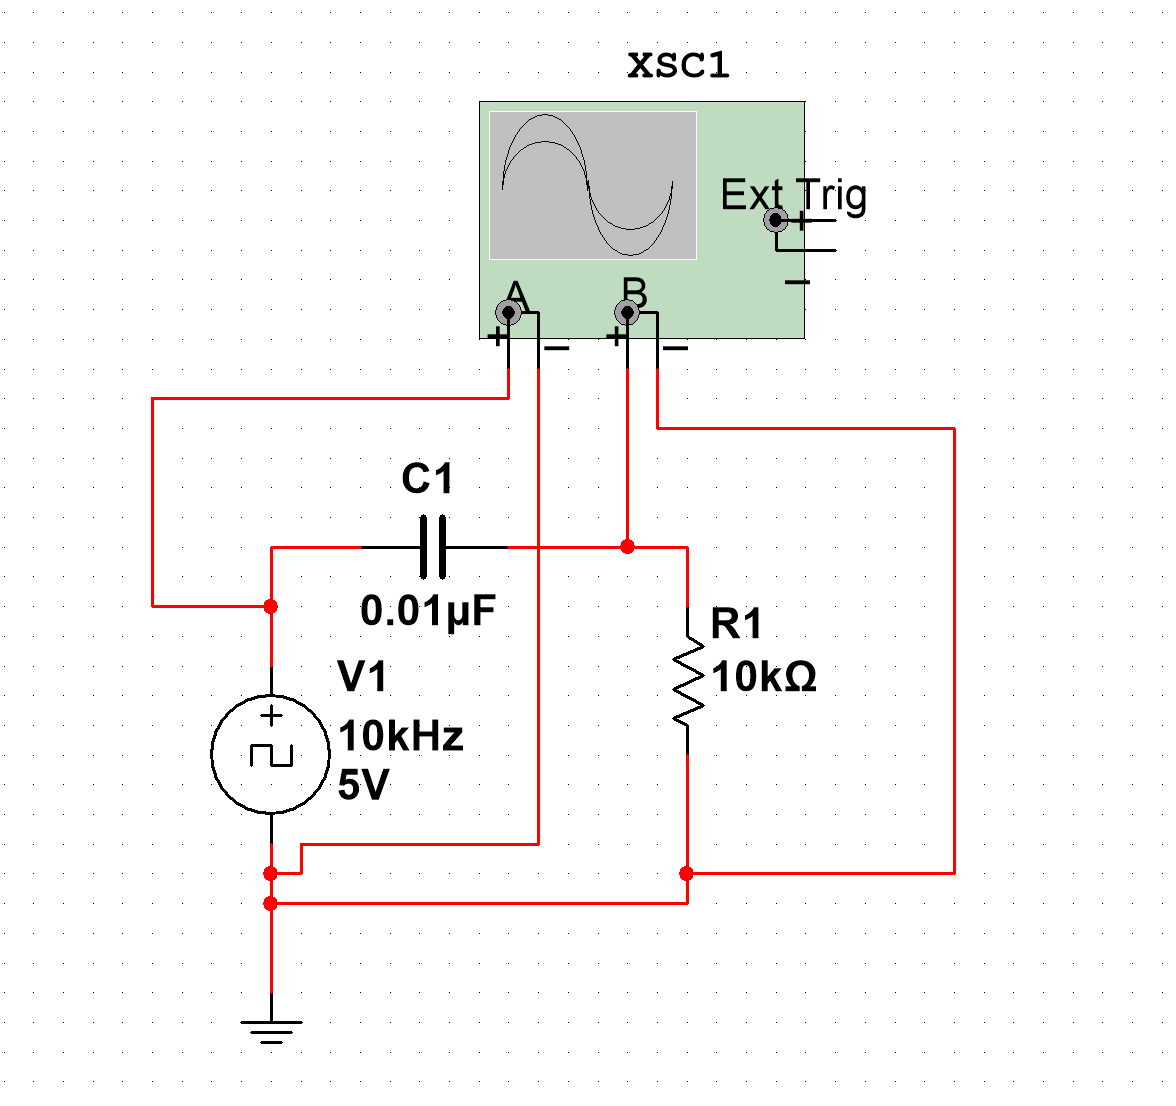
\includegraphics[width=0.68\textwidth]{rc_differentiator_multisim.png}
    \caption{微分电路 Multisim 仿真电路}
    \label{fig:rc-differentiator}
\end{figure}

\subsection{Multisim 仿真结果预期}

\begin{table}[H]
    \centering
    \caption{一阶 RC 电路仿真结果预期}
    \label{tab:simulation-expectation}
    \begin{tabular}{ll}
        \toprule
        项目 & 理论或仿真预期 \\
        \midrule
        时间常数 & \(\tau=RC=\SI{100}{\micro\second}\) \\
        充电到一个时间常数 & \(u_C(\tau)\approx0.632U_0\) \\
        放电到一个时间常数 & \(u_C(\tau)\approx0.368U_0\) \\
        积分电路输出 & 方波输入下输出为较平滑的斜坡或近似三角波 \\
        微分电路输出 & 方波上升沿和下降沿处产生正、负尖脉冲 \\
        \bottomrule
    \end{tabular}
\end{table}

% (10) 实验器件
\section{实验器件}

\begin{itemize}
    \item 面包板 \(\times 1\)
    \item 函数信号发生器 RIGOL DG922 \(\times 1\)
    \item 示波器 RIGOL DHO1204 \(\times 1\)
    \item 数字万用表 RIGOL DM858 \(\times 1\)
    \item 电阻：\(\SI{10}{\kilo\ohm}\times 1\)
    \item 电容：\(\SI{0.01}{\micro\farad}\times 1\)
    \item 导线若干
\end{itemize}

\end{document}
